% THIS IS SIGPROC-SP.TEX - VERSION 3.0
% WORKS WITH V3.1SP OF ACM_PROC_ARTICLE-SP.CLS
% JUNE 2007
%
% It is an example file showing how to use the 'acm_proc_article-sp.cls' V3.1SP
% LaTeX2e document class file for Conference Proceedings submissions.
% ----------------------------------------------------------------------------------------------------------------
% This .tex file (and associated .cls V3.1SP) *DOES NOT* produce:
%       1) The Permission Statement
%       2) The Conference (location) Info information
%       3) The Copyright Line with ACM data
%       4) Page numbering
% ---------------------------------------------------------------------------------------------------------------
% It is an example which *does* use the .bib file (from which the .bbl file
% is produced).
% REMEMBER HOWEVER: After having produced the .bbl file,
% and prior to final submission,
% you need to 'insert'  your .bbl file into your source .tex file so as to provide
% ONE 'self-contained' source file.
%
% Questions regarding SIGS should be to
% Adrienne Griscti ---> griscti@acm.org
%
% Questions/suggestions regarding the guidelines, .tex and .cls files, etc. to
% Gerald Murray ---> murray@acm.org
%
% For tracking purposes - this is V3.0SP - JUNE 2007

\documentclass{sig-alternate}

\usepackage{times}
\usepackage{graphicx}
\usepackage{epsf}
\usepackage{verbatim}
\usepackage{psfig}
\usepackage{cite}
\usepackage{url}
\usepackage{color}
\usepackage{alltt}

\usepackage{longtable,lscape}
\usepackage{slashbox,multirow}
\usepackage{colortbl}
\usepackage{mathrsfs}

\newcommand{\Add}{\CodeIn{add}}
\newcommand{\AVTree}{\CodeIn{AVTree}}
\newcommand{\Assignment}[3]{$\langle$ \Object{#1}, \Object{#2}, \Object{#3} $\rangle$}
\newcommand{\BinaryTreeRemove}{\CodeIn{BinaryTree\_remove}}
\newcommand{\BinaryTree}{\CodeIn{BinaryTree}}
\newcommand{\Caption}{\caption}
\newcommand{\Char}[1]{`#1'}
\newcommand{\CheckRep}{\CodeIn{checkRep}}
\newcommand{\ClassC}{\CodeIn{C}}
\newcommand{\CodeIn}[1]{{\small\texttt{#1}}}
\newcommand{\CodeOutSize}{\scriptsize}
\newcommand{\Comment}[1]{}
\newcommand{\Ensures}{\CodeIn{ensures}}
\newcommand{\ExtractMax}{\CodeIn{extractMax}}
\newcommand{\FAL}{field-ordering}
\newcommand{\FALs}{field-orderings}
\newcommand{\Fact}{observation}
\newcommand{\Get}{\CodeIn{get}}
\newcommand{\HashSet}{\CodeIn{HashSet}}
\newcommand{\HeapArray}{\CodeIn{HeapArray}}
\newcommand{\Intro}[1]{\emph{#1}}
\newcommand{\Invariant}{\CodeIn{invariant}}
\newcommand{\JUC}{\CodeIn{java.\-util.\-Collections}}
\newcommand{\JUS}{\CodeIn{java.\-util.\-Set}}
\newcommand{\JUTM}{\CodeIn{java.\-util.\-TreeMap}}
\newcommand{\JUTS}{\CodeIn{java.\-util.\-TreeSet}}
\newcommand{\JUV}{\CodeIn{java.\-util.\-Vector}}
\newcommand{\JMLPlusJUnit}{JML+JUnit}
\newcommand{\Korat}{Korat}
\newcommand{\Left}{\CodeIn{left}}
\newcommand{\Lookup}{\CodeIn{lookup}}
\newcommand{\MethM}{\CodeIn{m}}
\newcommand{\Node}[1]{\CodeIn{N}$_#1$}
\newcommand{\Null}{\CodeIn{null}}
\newcommand{\Object}[1]{\CodeIn{o}\ensuremath{_#1}}
\newcommand{\PostM}{\MethM$_{post}$}
\newcommand{\PreM}{\MethM$_{pre}$}
\newcommand{\Put}{\CodeIn{put}}
\newcommand{\Remove}{\CodeIn{remove}}
\newcommand{\RepOk}{\CodeIn{repOk}}
\newcommand{\Requires}{\CodeIn{requires}}
\newcommand{\Reverse}{\CodeIn{reverse}}
\newcommand{\Right}{\CodeIn{right}}
\newcommand{\Root}{\CodeIn{root}}
\newcommand{\Set}{\CodeIn{set}}
\newcommand{\State}[1]{2^{#1}}
\newcommand{\TestEra}{TestEra}
\newcommand{\TreeMap}{\CodeIn{TreeMap}}

\newenvironment{CodeOut}{\begin{scriptsize}}{\end{scriptsize}}
\newenvironment{SmallOut}{\begin{small}}{\end{small}}

\newcommand{\pairwiseEquals}{PairwiseEquals}
\newcommand{\monitorEquals}{MonitorEquals}
%\newcommand{\monitorWField}{WholeStateW}
\newcommand{\traverseField}{WholeState}
\newcommand{\monitorSMSeq}{ModifyingSeq}
\newcommand{\monitorSeq}{WholeSeq}

\newcommand{\IntStack}{\CodeIn{IntStack}}
\newcommand{\UBStack}{\CodeIn{UBStack}}
\newcommand{\BSet}{\CodeIn{BSet}}
\newcommand{\BBag}{\CodeIn{BBag}}
\newcommand{\ShoppingCart}{\CodeIn{ShoppingCart}}
\newcommand{\BankAccount}{\CodeIn{BankAccount}}
\newcommand{\BinarySearchTree}{\CodeIn{BinarySearchTree}}
\newcommand{\LinkedList}{\CodeIn{LinkedList}}

\newcommand{\Book}{\CodeIn{Book}}
\newcommand{\Library}{\CodeIn{Library}}

\newcommand{\Jtest}{Jtest}
\newcommand{\JCrasher}{JCrasher}
\newcommand{\Daikon}{Daikon}
\newcommand{\JUnit}{JUnit}

\newcommand{\trie}{trie}

\newcommand{\Perl}{Perl}


\newcommand{\SubjectCount}{11}
\newcommand{\DSSubjectCount}{two}

\newcommand{\Equals}{\CodeIn{equals}}
\newcommand{\Pairwise}{PairwiseEquals}
\newcommand{\Subgraph}{MonitorEquals}
\newcommand{\Concrete}{WholeState}
\newcommand{\ModSeq}{ModifyingSeq}
\newcommand{\Seq}{WholeSeq}
\newcommand{\Aeq}{equality}

\newcommand{\Meaning}[1]{\ensuremath{[\![}#1\ensuremath{]\!]}}
\newcommand{\Pair}[2]{\ensuremath{\langle #1, #2 \rangle}}
\newcommand{\Triple}[3]{\ensuremath{\langle #1, #2, #3 \rangle}}
\newcommand{\SetSuch}[2]{\ensuremath{\{ #1 | #2 \}}}

\newcommand{\Equiv}[2]{\ensuremath{#1 \EquivSTRel{} #2}}
\newcommand{\EquivME}{\Equiv}
\newcommand{\EquivST}{\Equiv}
\newcommand{\EquivSTRel}{\ensuremath{\cong}}
\newcommand{\Redundant}[2]{\ensuremath{#1 \lhd #2}}
\newcommand{\VB}{\ensuremath{\mid}}
\newcommand{\MES}{method-entry state}

\newcommand{\Small}[1]{{\small{#1}}}

\newcommand{\CenterCell}[1]{\multicolumn{1}{c|}{#1}}


\begin{document}

\conferenceinfo{ESEC-FSE'09,} {August 23--28, 2009, Amsterdam, The Netherlands.} 
\CopyrightYear{2009}
\crdata{978-1-60558-001-2/09/08} 

\title{MSeqGen: Object-Oriented Unit-Test Generation via Mining Source Code\titlenote{This work is supported in part by NSF grant CCF-0725190 and Army Research Office grant W911NF-08-1-0443.}}
%
% You need the command \numberofauthors to handle the 'placement
% and alignment' of the authors beneath the title.
%
% For aesthetic reasons, we recommend 'three authors at a time'
% i.e. three 'name/affiliation blocks' be placed beneath the title.
%
% NOTE: You are NOT restricted in how many 'rows' of
% "name/affiliations" may appear. We just ask that you restrict
% the number of 'columns' to three.
%
% Because of the available 'opening page real-estate'
% we ask you to refrain from putting more than six authors
% (two rows with three columns) beneath the article title.
% More than six makes the first-page appear very cluttered indeed.
%
% Use the \alignauthor commands to handle the names
% and affiliations for an 'aesthetic maximum' of six authors.
% Add names, affiliations, addresses for
% the seventh etc. author(s) as the argument for the
% \additionalauthors command.
% These 'additional authors' will be output/set for you
% without further effort on your part as the last section in
% the body of your article BEFORE References or any Appendices.

\numberofauthors{1} %  in this sample file, there are a *total*
% of EIGHT authors. SIX appear on the 'first-page' (for formatting
% reasons) and the remaining two appear in the \additionalauthors section.
%

\author{Suresh Thummalapenta$^1$, Tao Xie$^1$, Nikolai Tillmann$^2$, Jonathan de Halleux$^2$, Wolfram Schulte$^2$\\
\affaddr{$^1$Department of Computer Science, North Carolina State University, Raleigh}\\
\affaddr{$^2$Microsoft Research, One Microsoft Way, Redmond}\\
\email{$^1$\{sthumma, txie\}@ncsu.edu, $^2$\{nikolait, jhalleux, schulte\}@microsoft.com}\\
}

%\author{
% You can go ahead and credit any number of authors here,
% e.g. one 'row of three' or two rows (consisting of one row of three
% and a second row of one, two or three).
%
% The command \alignauthor (no curly braces needed) should
% precede each author name, affiliation/snail-mail address and
% e-mail address. Additionally, tag each line of
% affiliation/address with \affaddr, and tag the
% e-mail address with \email.
%
% 1st. author
%\alignauthor
%Suresh Thummalapenta\\
%       \affaddr{Department of Computer Science}\\
%       \affaddr{North Carolina State University}\\
%       \affaddr{Raleigh, USA}\\
%       \email{sthumma@ncsu.edu}
%% 2nd. author
%\alignauthor
%Tao Xie\\
%			 \affaddr{Department of Computer Science}\\
%       \affaddr{North Carolina State University}\\
%       \affaddr{Raleigh, USA}\\
%       \email{xie@csc.ncsu.edu}% 3rd. author
%\and
%\alignauthor Nikolai Tillmann, Jonathan de Halleux, Wolfram Schulte\\
%       \affaddr{Microsoft Research}\\
%       \affaddr{One Microsoft Way, Redmond, USA}\\
%       \email{\{nikolait, jhalleux, schulte\}@microsoft.com}  
%}

\maketitle
\begin{abstract}
An objective of unit testing is to achieve high structural coverage of the code under test. Achieving high structural coverage of object-oriented code requires desirable method-call sequences that create and mutate objects. These sequences help generate target object states such as argument or receiver object states (in short as target states) of a method under test. Automatic generation of sequences for achieving target states is often challenging due to a large search space of possible sequences. On the other hand, code bases using object types (such as receiver or argument object types) include sequences that can be used to assist automatic test-generation approaches in achieving target states. In this paper, we propose a novel approach, called $\smoot$, that mines code bases and extracts sequences related to receiver or argument object types of a method under test. Our approach uses these extracted sequences to enhance two state-of-the-art test-generation approaches: random testing and dynamic symbolic execution. We conduct two evaluations to show the effectiveness of our approach. Using sequences extracted by our approach, we show that a random testing approach achieves 8.7\% (with a maximum of 20.0\% for one namespace) higher branch coverage and a dynamic-symbolic-execution-based approach achieves 17.4\% (with a maximum of 22.5\% for one namespace) higher branch coverage than without using our approach. Such an improvement is significant as the branches that are not covered by these state-of-the-art approaches are generally quite difficult to cover.
\end{abstract}

\vspace{1mm} \noindent {\bf Categories and Subject Descriptors:}
D.2.3 {[Software Engineering]}: {Coding Tools and
Techniques---\emph{Object-oriented programming}}; D.2.6 {[Software Engineering]}: {Programming
Environments---\emph{Integrated environments}};

\vspace{1mm} \noindent {\bf General Terms:} Languages,
Experimentation

\vspace{1mm} \noindent {\bf Keywords:} Object-oriented testing, Sequence mining

\section{Introduction}
\label{sec:intro}
\vspace*{-3ex}
Programming languages such as Java and C++ provide exception-handling 
constructs such as \CodeIn{try-catch} to handle exception conditions that arise
during program execution. Under these exception conditions, programs follow paths
different from normal execution paths; these additional paths are referred to as 
\emph{exception} paths. Applications developed based on these programming
languages are expected to handle these exception conditions and take necessary recovery
actions. For example, when an application reuses resources such as files or database connections,
the application should release the resources after the usage in all paths
including \Intro{exception} paths. Failing to release the resources can not only cause performance degradation, 
but can also lead to critical issues. For example, if a database lock acquired by a
process is not released, any other process trying to acquire the same lock
hangs till the database releases the lock after timeout.
A case study~\cite{Weimer04} conducted on a real application 
demonstrates the necessity of releasing resources in exception paths 
for improving reliability and performance. 
The case study found that there was a surprising
improvement of 17\% in performance of the application after 
correctly releasing resources in the presence of exceptions.

\Comment{In general, software verification concentrates on verifying behaviors of the application 
during normal execution paths rather than exception paths. Therefore, the exception 
cases remain undetected during traditional software verification.}

Software verification can be challenging for exception cases as verification
techniques require specifications that describe expected behaviors when exceptions occur.
These specifications are often not available in practice~\cite{document:leth}.
To address this issue, association rules of the form ``$FC_a$ $\Rightarrow$ $FC_e$''
are mined as specifications~\cite{WeimerN05}, where both $FC_a$ and $FC_e$ are function calls that share
the same receiver object. These specifications are used to 
verify whether the function call $FC_a$ is followed by the function call $FC_e$ in all 
exception paths. However, simple association rules of this form are often not sufficient
to characterize common exception-handling rules. The rationale is that
there are various scenarios where $FC_a$ is not necessarily followed by $FC_e$ 
when exceptions are raised by $FC_a$, although both function calls 
share the same receiver object. 

\begin{figure*}[t]
\centering
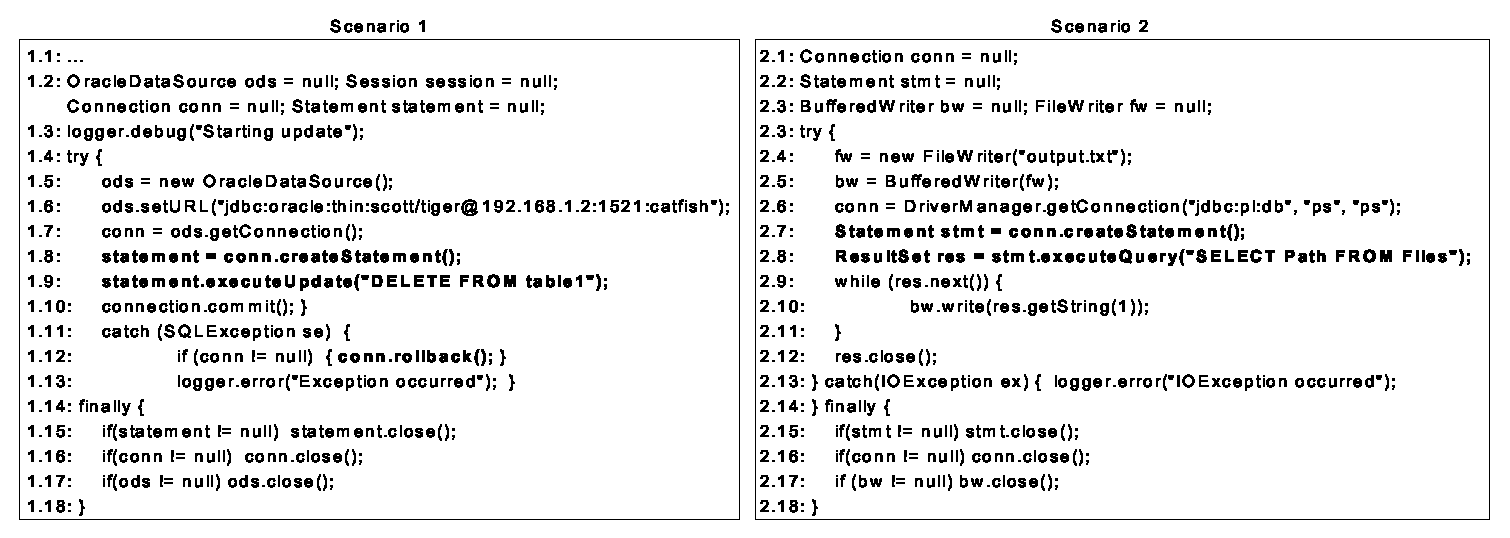
\includegraphics[scale=0.70,clip]{figs/three-code-examples1.eps}\vspace*{-3ex}
\centering \caption {\label{fig:threescenarios} Two example scenarios from real applications.}\vspace*{-4ex}
\end{figure*}

We next present an example using Scenarios 1 and 2 (extracted 
from real applications) shown in Figure~\ref{fig:threescenarios}. 
Scenario 1 attempts to modify contents of a database through the function call
\CodeIn{Statement.executeUpdate} (Line 1.9), whereas Scenario 2 attempts to read contents
of a database through the function call \CodeIn{Statement.executeQuery} (Line 2.8).
Consider a simple specification in the form of an association
rule ``\CodeIn{Connection creation} $\Rightarrow$
\CodeIn{Connection rollback}''. This rule describes that a \CodeIn{rollback} function call should
appear in exception paths whenever an object of \CodeIn{Connection} is created. 
Although a \CodeIn{Connection} object is created in both
scenarios, this rule applies only to Scenario 1 and does not apply to Scenario 2.
The primary reason is that the \CodeIn{rollback} function call should be invoked \emph{only} when 
there are any changes made to the database. This example shows that
simple association rules of the form ``$FC_a$ $\Rightarrow$ $FC_e$''
are often insufficient to characterize exception-handling rules.

The insufficiency of simple association rules calls for 
more general association rules, hereby referred to as \Intro{sequence association rules},
of the form ``($FC_c^1$...$FC_c^n$) $\wedge$ $FC_a$ $\Rightarrow$ ($FC_e^1$...$FC_e^m$)''.
This sequence association rule describes that function call $FC_a$ should be followed 
by function-call sequence $FC_e^1$...$FC_e^m$ in exception paths only 
when preceded by function-call sequence $FC_c^1$...$FC_c^n$. Using this sequence association rule,
the preceding example can be expressed as ``($FC_c^1$$FC_c^2$) $\wedge$ 
$FC_a$ $\Rightarrow$ ($FC_e^1$)'', where

$FC_c^1$ : \CodeIn{OracleDataSource.getConnection}\\
\hspace*{0.15in}$FC_c^2$ : \CodeIn{Connection.createStatement}\\
\hspace*{0.15in}$FC_a$ : \CodeIn{Statement.executeUpdate}\\
\hspace*{0.15in}$FC_e^1$ : \CodeIn{Connection.rollback}\\
\vspace*{-2ex}

This sequence association rule applies to Scenario 1 and
does not apply to Scenario 2 due to the presence of $FC_a$: \CodeIn{Statement.executeUpdate}.
The key aspects to be noted in this rule are: (1) \CodeIn{Statement.executeUpdate}
is the primary reason to have \CodeIn{Connection.rollback} in an exception path and
(2) the receiver object of \CodeIn{Statement.executeUpdate} is dependent on the 
receiver object of \CodeIn{Connection.rollback} through the function-call sequence
defined by $FC_c^1$$FC_c^2$.

Our sequence association rules are a super set of simple association rules.
For example, sequence association rules are the same as simple association
rules when the sequence $FC_c^1$...$FC_c^n$ is empty. 
To the best of our knowledge, existing association rule mining techniques~\cite{agarwal:association}
cannot be directly applied to mine these sequence association rules. 
Therefore, to bridge the gap, we develop a new mining algorithm by adapting the
frequent closed subsequence mining technique~\cite{wang:bide}. 

We further develop a novel approach, called CAR-Miner, that incorporates
our new mining algorithm for the problem of detecting exception-handling rules in
the form of sequence association rules by analyzing source code. Apart from mining sequence
association rules, CAR-Miner addresses another challenge that is often faced 
by existing approaches~\cite{Zhenmin2005PRMiner, chang07:finding, WeimerN05}, 
which mine rules from a limited data scope, 
i.e., from only a few example applications. Therefore, these approaches may not 
be able to mine rules that do not have enough
supporting samples in those example applications, and hence 
the related defects remain undetected by these approaches. To address
this challenge, CAR-Miner expands the data scope by leveraging a code search engine (CSE)
for gathering relevant code samples from existing open source projects available
on the web. From these relevant code samples, CAR-Miner mines exception-handling rules. 
We show the usefulness of mined exception-handling rules
by applying these rules on five applications to detect violations.
CAR-Miner tries to address problems related to the quality of code samples 
gathered from a CSE by capturing the most frequent patterns through mining.

\Comment{In particular, CAR-Miner accepts an input application and tries to detect
exception-handling defects in that application. Initially, CAR-Miner gathers function calls, referred as
$FC_a$, used by  the input application. CAR-Miner interacts with a code search engine (CSE) such as Google code search~\cite{GCSE} to gather related code examples that are already reusing $FC_a$. 
CAR-Miner constructs an Exception Flow Graph (EFG) for each code example gathered from 
the CSE. EFG is an extended form of control flow graph that captures flow of control in both
normal and exception conditions. While constructing EFG, we add only those exception
paths that can occur potentially during program execution. To capture such
exception paths, we use a sound static analysis that provides a set
of exceptions thrown by each $FC_a$ during program execution. 
CAR-Miner collects traces, which are
in the form of a sequence of function calls, from EFG post-processes these 
traces to filter unrelated function calls of $FC_a$.
CAR-Miner mines these traces to capture sequence association rules. 
Finally, CAR-Miner applies mined exception-handling rules to detect violations in the input application.
As CAR-Miner leverages a code search engine for gathering related code examples,
CAR-Miner has an added advantage of being able to mine rules, which do not have enough
supporting samples in the input application. CAR-Miner tries to address the 
problems related to the quality of the code examples 
gathered from a CSE by capturing the most frequent rule candidates through mining.}

This paper makes the following main contributions:\vspace*{-1ex}
\begin{Itemize}
\item A general mining algorithm to mine sequence association rules of the form 
``($FC_c^1$...$FC_c^n$) $\wedge$ $FC_a$ $\Rightarrow$ ($FC_e^1$...$FC_e^m$)''.
Our new mining algorithm takes a step forward in the direction 
of developing new mining algorithms to address
unique requirements in mining software engineering data, beyond being limited
by existing off-the-shelf mining algorithms.\vspace*{-2ex}
\item An approach that incorporates the general mining algorithm to mine exception-handling
rules that describe expected behavior when exceptions occur during
program execution. \vspace*{-2ex}
\item A technique for constructing a precise Exception-Flow Graph (EFG), which is an extended form of 
a Control-Flow Graph (CFG), that includes only those exception paths that can potentially occur 
during program execution.\vspace*{-2ex}
\item An implementation for expanding the data scope to open source projects that help
detect new related exception-handling rules that do not have enough supporting samples in an application under analysis.
These rules can help detect new defects in the application under analysis.\vspace*{-2ex}
\item Two evaluations to show
the effectiveness of our approach. (1) CAR-Miner detects $294$ real 
exception-handling rules in five different applications including $285$ KLOC. 
(2) The top $50$ exception-handling
rules (top $10$ real rules of each application)
are used to detect a total of $160$ real defects in these five
applications, where $87$ defects are new, not being detected by a 
previous related approach~\cite{WeimerN05}. \Comment{The initial response from 
developers of HsqlDB~\footnote{\url{http://hsqldb.sourceforge.net/}} is
encouraging. The developers responded on the first ten defects that we reported, 
where seven defects are \emph{accepted} and only three defects are rejected.}
\end{Itemize}

The rest of the paper is organized as follows. 
%Section~\ref{sec:example} presents example scenarios.
Section~\ref{sec:condrules} presents a formal definition of sequence
association rules and describes our new mining algorithm.
Section~\ref{sec:approach} describes key aspects of the CAR-Miner approach.
Section~\ref{sec:eval} presents evaluation results.
%Section~\ref{sec:discussion} presents limitations and future work.
Section~\ref{sec:threats} discusses threats to validity.
Section~\ref{sec:related} presents related work.
Finally, Section~\ref{sec:conclusion} concludes.


\section{Background}
\label{sec:background}

We next provide details of two major concepts used in the rest of
the paper: dynamic symbolic execution and dynamic code coverage.

%-----------------------------------------------------------------------------
\subsection{Dynamic Symbolic Execution}

In our approach, we use Pex as an example state-of-the-art dynamic symbolic 
execution tool. Pex~\cite{tillman:pexwhite} is an automatic unit-test-generation 
tool developed by Microsoft. Pex accepts PUTs as input and generates conventional 
unit tests that can achieve high 
structural coverage of the code under test. Initially, Pex
executes the code under test with random inputs. While executing
the code under test, Pex collects constraints on inputs from predicates
in branching statements. Pex next solves collected constraints
to generate new test inputs that guide future executions along
new paths. Pex includes various optimization techniques such as
reducing the size of the formula before giving it over constraint solver.

%-----------------------------------------------------------------------------
\subsection{Dynamic Code Coverage}

In this paper, we use Pex generated reports for measuring coverage. These coverage
reports are called dynamic, because Pex knows only about the code that was already executed.
As Pex is not aware of the code that is not yet executed, dynamic code coverage
cannot give absolute values for the coverage. The primary reason for using
dynamic code coverage in our paper is that C\# allows generate code during run time.
Therefore, it is often not possible to find out how much code exists beforehand.
\section{Example}
\label{sec:example}

TeMAPI includes three major steps in detecting behavioral differences among API elements described in mapping relations. We use JLCA (a Java-to-C\# translation tool) as an example translation tool, and the \CodeIn{java.io.ByteArrayInputStream} class in Java as an example API element to illustrate these three steps.

%----------------------------------------------------
\textbf{Translating Synthesized wrappers.} TeMAPI first synthesizes a Java wrapper class for the example class. TeMAPI next uses JLCA to translate the wrapper class to C\#. TeMAPI compares source code of the synthesized wrapper class with the translated wrapper class to extract translatable API elements of the example class. In particular, our example class in Java has five fields, two constructors, and eight methods besides inherited ones\footnote{\url{http://tinyurl.com/2dsgftv}}. A class can have more than one constructor, and a translation tool may not translate all its constructors. Therefore, to address this issue, TeMAPI includes different constructors in its synthesized wrapper methods instead of simply pushing the receiver object as a parameter of wrapper methods. For example, TeMAPI first identifies \CodeIn{ByteArrayInputStream(byte[])} constructor as translatable, and synthesizes the wrapper method for the \CodeIn{skip(long)} method as follows:

\begin{CodeOut}\vspace*{-1ex}
\begin{alltt}
public long testskip24nm(long m0, byte c0[])\{
  ByteArrayInputStream obj = new ByteArrayInputStream(c0);
  return obj.skip(m0);\}
\end{alltt}
\end{CodeOut}\vspace*{-2ex}

TeMAPI next uses JLCA to translate synthesized wrapper methods from Java to C\#. A translation tool typically cannot include mapping relations for all the API elements between two languages, so translated wrapper methods can have compilation errors. TeMAPI parses translated wrapper methods and filters out all methods with compilation errors. For example, below is the translated \CodeIn{testskip- 24nm} method in C\#:
\vspace*{-2ex}

\begin{CodeOut}
\begin{alltt}
public virtual long testskip24nm(long m0, sbyte[] c0)\{
  MemoryStream obj = new MemoryStream(
                    SupportClass.ToByteArray(c0));
  MemoryStream temp_BufferedStream = obj;
  Int64 temp_Int64 = temp_BufferedStream.Position;
  temp_Int64 = temp_BufferedStream.Seek(m0,
       System.IO.SeekOrigin.Current) - temp_Int64;
  return temp_Int64;\}
\end{alltt}
\end{CodeOut}\vspace*{-2ex}

TeMAPI does not remove this method, since it does not result in compilation errors.


\textbf{Generation of C\# Test Cases for Testing Java Code.} A major advantage of our synthesized wrapper is that the original wrapper and the translated wrapper shares the same interface, irrespective of method calls within the wrapper method. Therefore, TeMAPI detects behavioral differences between mapped API elements by generating test cases on one version of wrapper methods and applying those test cases on the other version. In particular, TeMAPI extends Pex~\cite{tillmann2008pex} to generate test cases for each remaining C\# wrapper method. For the example class, Pex attempts to explore all feasible paths among method calls within the wrapper methods and generates inputs and outputs that exercise various paths. Based on the inputs and output generated for each path, TeMAPI generates a Java test case to check whether the original wrapper method return the same values as the translated one. For example, TeMAPI generates the following Java test case based on inputs generated by Pex for one feasible path (in the C\# wrapper method) that throws exceptions.

\begin{CodeOut}\vspace*{-1ex}
\begin{alltt}
public void testskip24nm36()\{
  try\{
     Test_java_io_ByteArrayInputStream obj =
        new Test_java_io_ByteArrayInputStream();
     long m0 = java.lang.Long.valueOf(
                  "2147483648").longValue();
     byte[] c0 = new byte[0];
     obj.testskip24nm(m0,c0);
     Assert.assertTrue(false);
  \}catch(java.lang.Exception e)\{
     Assert.assertTrue(true); \}\}
\end{alltt}
\end{CodeOut}\vspace*{-2ex}

This Java test case fails, since given the preceding inputs, the \CodeIn{skip (long)} method in Java does not throw any exceptions, instead the translated C\# code does. Thus, TeMAPI detects a behavioral difference between the \CodeIn{skip(long)} method in Java and its translated C\# API elements by JLCA.

%-----------------------------------
\textbf{Generation of Java Test Cases for Testing C\# Code.} As shown by Thummalapenta \emph{et al.}~\cite{thummalapenta09:mseqgen}, Pex cannot effectively generate sequences. To address this issue, TeMAPI extends Randoop~\cite{pacheco2007feedback} for testing Java code to generate invocation sequences. TeMAPI does not generate invocation sequences from wrappers directly, since each wrapper method includes a fixed simple invocation sequence. Instead, TeMAPI uses translatable API methods in Step 1, and limits the scope of Randoop to those methods while generating invocation sequences. For example, a generated Java test case is as follows:

\begin{CodeOut}\vspace*{-1ex}
\begin{alltt}
public void test413() throws Throwable\{
  ...
  ByteArrayInputStream var2=new ByteArrayInputStream(...);
  var2.close();
  int var5=var2.available();
  assertTrue(var5 == 1);\}
\end{alltt}
\end{CodeOut}\vspace*{-2ex}


The test case gets passed, since Java allows access to the stream even if the stream is closed. TeMAPI next uses JLCA to translate the generated Java test case from Java to C\#. Since the Java test case uses only translatable API elements, JLCA translates the test case to a C\# test case as follows:

\begin{CodeOut}\vspace*{-1ex}
\begin{alltt}
public void test413() throws Throwable\{
  ...
  MemoryStream var2 = new MemoryStream(...);
  var2.close();
  long available = var2.Length - var2.Position;
  int var5 = (int) available;
  AssertTrue(var5 == 1);\}
\end{alltt}
\end{CodeOut}\vspace*{-2ex}

In contrast to the Java test case, the C\# test case gets failed since C\# does not allow such access to the stream and throws \CodeIn{ObjectDis\\posedException}. TeMAPI thus detects a behavioral difference with invocation sequences.

This example motivates our basic idea of generating test cases in one language and translating those test cases to another language for detecting differences among API mapping relations. %We next present details of our approach.

%\begin{figure}[t]
%\centering %\hfill
%\includegraphics[scale=0.95,clip]{figure/sample.eps}\vspace*{-3ex}
% \caption{\label{fig:example}API mapping}\vspace*{-4ex}
%\end{figure}

%Based on the mapping relations, a translation tool can migrate the
%preceding code snippet automatically. To learn the mapping
%relations,
%
%%\begin{figure}[t]
%%\centering
%%\includegraphics[scale=0.86,clip]{figure/openfile.eps}\vspace*{-1.5ex}
%% \caption
%%{\label{fig:openfile}Aligned wrapper}\vspace*{-2ex}
%%\end{figure}
%
%In this section, we illustrate the main steps of MAM to
%mine the API mapping in Java for \CodeIn{System.IO.Directory.
%Exists()} in C\# from the HypoLog
%project\footnote{\url{http://sourceforge.net/projects/twlog/}}.
%
%The first step of MAM is to align classes and methods of
%wrapper by names. This step finds class pairs and method pairs
%that implement similar functionalities, and each pair may use
%API mapping since it implements a similar functionality. Our
%approach chooses names to align classes and methods because these
%classes and methods are from the same project. In this example, our
%approach aligns the two methods as shown in
%Figure~\ref{fig:openfile} because the two method have similar names
%and their declaring classes also have similar names (see
%Section~\ref{sec:approach:alignclientcode} for details).
%
%The second step of MAM is to mine mapping relations of API
%classes based on the names of corresponding fields, parameters,
%returned types, and local variables. This step also relies on names
%for the same consideration of the first step. For example, our
%approach maps the two parameters with the same name as shown by the
%red arrow of Figure~\ref{fig:openfile}. From the types of the two
%parameters, MAM mines the mapping relation between two API
%classes: \CodeIn{System.String} $\leftrightarrow$
%\CodeIn{java.lang.String} (see
%Section~\ref{sec:approach:mappingtypes} for details).
%
%
%The final step of MAM is to mine mapping relations of API
%methods. Besides the factors listed in
%Section~\ref{sec:introduction}, another factor is that API calls in
%wrapper are often not carefully aligned. To deal with those
%challenges, MAM first builds an API Transformation Graph
%(ATG) for each method. After that, MAM compares built
%graphs to mine mapping relations of API methods (see
%Section~\ref{sec:approach:mappingtypes} and
%Figure~\ref{fig:approach1} for details). Figure~\ref{fig:example}
%shows the mined mapping relation between
%\CodeIn{System.IO.Directory.Exists()} and its API mapping in
%Java.

\section{Approach}
\label{sec:approach}

Our approach accepts a set of projects as data sources and mines
API mapping between two different languages $L_1$ and $L_2$.
As mined API mapping describes mapping relations of APIs between
the two languages, this mapping is useful for language migration between the two languages.
For each project used as a data source, our approach requires
atleast two versions of the project (one version in $L_1$ and
the other version in $L_2$). Figure~\ref{fig:approach} shows
the overview of our approach.

First, our approach aligns client code in languages $L_1$ and $L_2$
so that the aligned source files implement similar functionalities
(Section~\ref{sec:approach:acc}). Second, our approach mines
mapping relations of API classes (Section~\ref{sec:approach:mappingtypes}).
Finally, our approach mines mapping relations of API
methods (Section~\ref{sec:approach:mappingtypes}) defined by the mapped
API classes.

\begin{figure}[t]
\centering
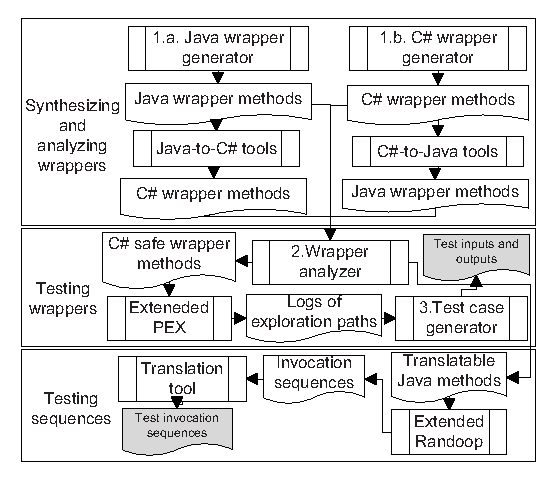
\includegraphics[scale=1,clip]{figure/approach.eps}\vspace*{-3ex}
 \caption{Overview of our approach}\vspace*{-3.5ex}
 \label{fig:approach}
\end{figure}

%-------------------------------------------------------------------
\subsection{Aligning Client Code}
\label{sec:approach:acc}

Initially, our approach accepts two versions of a project (one version in
$L_1$ and the other version in $L_2$) and aligns classes and methods
of the two versions. Aligned classes or methods
between the two versions implement a similar functionality. As they
implement a similar functionality, APIs used by these classes or methods can be
replaceable.

To align classes and methods of the two versions, our approach uses
name similarities between entities (such as class names or method names)
defined by the two versions of the project. In our approach, we have two
different kinds of entity names: entity names defined by the two versions
of the project and entity names of third-party libraries used by the two versions of the project.
The first kind often comes from the same programmer or the same team, or
programmers may refer to existing versions for naming entities such
as classes, methods, and variables. Therefore, name similarity is often
reliable to distinguish functionalities of the first kind compared to the second
kind. Our approach uses Simmetrics\footnote{\url{http://sourceforge.net/projects/simmetrics/}}
to calculate name similarities.

Algorithm 1 shows how our approach aligns client code classes. The
first step is to find candidate class pairs by names. For two sets
of classes ($C$ and $C'$), the algorithm returns candidate class
pairs ($M$) with a similarity greater than a given threshold,
referred to as \emph{SIM\_THRESHOLD}. As some projects may have many
classes with the same name, $M$ may contain more than one matching
pair for a class in a version. To align those classes, our algorithm
uses package names of these classes to refine $M$ and returns only
one matching pair with the maximum similarity\footnote{For C\#, we
refer to namespace names for package names.}.

In each aligned class pair, our approach further aligns methods
within the class pair. The algorithm for methods is similar to the
algorithm for classes but relies on other criteria such as the number of parameters
and names of parameters to refine candidate method pairs. These candidates
may contain more than one method pair due to overloading.
For the example shown in Section~\ref{sec:example}, our approach
correctly aligns the class \CodeIn{IndexFiles} and the method
\CodeIn{main} in Java to the class \CodeIn{IndexFiles}
and the method \CodeIn{Main} in C\# as their names are quite
similar.
%-----------------------------------------------------------------
\subsection{Mapping API classes}
\label{sec:approach:mappingtypes}

In this step, our approach mines mapping relations of
API classes. As defined in Section~\ref{sec:mapping}, mapping relations of API classes are used
to translate variables. Consequently, our approach mines mapping
relations of API classes based on how aligned client code declares
variables such as fields of aligned classes, parameters of aligned methods
and local variables of aligned methods. In
particular, for each aligned class pair $\Pair{c_1} {c_2}$, our
approach analyzes each field pair $\Pair{f_1}{f_2}$ and considers
$\Pair{f_1.type} {f_2.type}$ as one mined mapping relation of API
classes when the similarity between $f_1.name$ and $f_2.name$ is
greater than \emph{SIM\_THRESHOLD}. Similarly, for each aligned method pair
$\Pair{m_1} {m_2}$, our approach analyzes each local variable pair
$\Pair{var_1} {var_2}$ and considers $\langle var_1.type,$ $
var_2.type\rangle$ as one mined mapping relation of API classes when
the similarity between $var_1.name$ and $var_2.name$ is greater than
a threshold. Also, our approach analyzes each parameter pair
$\langle para_1, $ $para_2\rangle$ of $m_1$ and $m_2$, and our
approach considers $\langle para_1.type,$ $para_2.type\rangle$ as
one mined mapping relation of API classes when the similarity
between $para_1.name$ and $para_2.name$ is greater than \emph{SIM\_THRESHOLD}.

For the example shown in Section~\ref{sec:example}, our approach
mines the mapping relation between \CodeIn{java.io.File} and
\CodeIn{System.IO.FileInfo} based on the matched fields of Lines 4
and 9 (Figure~\ref{fig:clientcode}). The mapping relation of API classes helps translate the
variable declared in Line 1 (Figure~\ref{fig:totranslation})
to the variable declared in Line 16 (Figure~\ref{fig:translatedcode}).

%\begin{algorithm}[t]
%\begin{SmallOut}
%\dontprintsemicolon
%  \KwIn{$C$ is the classes of a language; $C'$ is the classes
%  of another language}
%  \KwOut{$P$ is aligned pairs of classes}
%  \Begin{
%     $M \leftarrow findCandidateClassPairs(C, C')$\;
%     \While{$M.size > 0 $}{
%        \If{$M.size > 1$}{
%            $M \leftarrow refineByPackageNames(M)$\;
%         }
%         \If{$M.size == 1$}{
%                $P.add(M)$\;
%                $C.remove(M[0].c)$\;
%                $C'.remove(M[0].c')$\;
%         }
%         $M \leftarrow findCandidateClassPairs(C, C')$\;
%     }
% }
%\end{SmallOut}
%\label{alg:alignclasses} \caption{Align Classes Algorithm}
%\end{algorithm}

\begin{figure}[t]
\centering
\includegraphics[scale=1,clip]{figure/algorithm1.eps}
\vspace*{-6ex}
\end{figure}

%-----------------------------------------------------------
\subsection{Mapping API methods}
\label{sec:approach:mappingtypes}

In this step, our approach mines mapping relations of API methods.
This step has two major sub-steps. First, our approach builds a graph, referred
as API transformation graph, for each client code
method. Second, our approach compares the two graphs of each paired
client code methods for mining mapping relations of API methods.

\begin{figure*}[t]
\centering
\includegraphics[scale=1.1,clip]{figure/graph.eps}\vspace*{-3ex}
 \caption
{\label{fig:graph}Built ATGs and the main steps of comparing
ATGs}\vspace*{-3.5ex}
\end{figure*}


\subsubsection{API transformation graph}
We propose API transformation graphs (ATG) to help deal with the two
challenges of mining API mapping listed in
Section~\ref{sec:introduction}. An API transformation graph of a
client code method $m$ is a directed graph
$G\Triple{N_{data}}{N_{m}}{E}$. $N_{data}$ is a set of the fields
$F$ of $m$'s declaring class, local variables $V$ of $m$, parameters
$P_1$ of $m$, parameters $P_2$ of methods called by $m$, and return
values $R$ of all methods. $N_{m}$ is a set of methods called by
$m$. $E$ is a set of directed edges. An edge $d_1\rightarrow d_2$
from a datum $d_1 \in N_{data}$ to a datum $d_2 \in N_{data}$
denotes the data dependency from $d_1$ to $d_2$. An edge $d_1
\rightarrow m_1$ from a datum $d_1 \in N_{data}$  to a method $ m_1
\in N_{m}$ denotes $d_1$ is a parameter or a related variable of
$m_1$. An edge $m_1 \rightarrow d_1$ from a method $m_1 \in N_{m}$
to a datum $d_1 \in N_{data}$ denotes $d_1$ is the return value of
$m_1$.

%We propose ATG for two main purposes. The first purpose is to mine mapping
%relations among parameters of mapped API methods. Mining mapping relations
%among parameters of mapped API methods is challenging as often mapped API methods
%can have different number of parameters or different positions among
%parameters. For example, consider the following two mapped API methods:
%
%\begin{CodeOut}
%$m_1$ in Java: BigDecimal java.math.BigDecimal.multiply (BigDecimal $p_1^1$)\\
%\hspace*{0.11in}$m_2$ in C\#: Decimal System.Decimal.Multiply (Decimal $p_1^2$, Decimal $p_2^2$)
%\end{CodeOut}
%
%Method $m_1$ of Java has a receiver variable, say $v_1^1$, of type \CodeIn{BigDecimal}
%and has one parameter $p_1^1$. The mapped method $m_2$ in C\# has
%two parameters $p_1^2$ and $p_2^2$. Using ATGs, our approach
%identifies that $v_1^1$ is mapped to $p_1^2$ and $p_1^1$ is mapped
%to $p_2^2$. As ATG captures parameters of API methods,
%our approach is able to deal with the challenges of mapping parameters.
%
%The second purpose of ATG is to mine mapping relations of merged API methods. As ATG
%describes data dependencies among inputs and outputs, our approach
%is able to mine mapping relations for merged API methods as shown in
%Figure~\ref{fig:example}. We next describe how our approach builds ATGs and
%uses ATGs for mining mapping relations of API methods.

\subsubsection{Building API transformation graphs }

Our approach builds an ATG for each method $m$. ATG includes information such as
inputs and outputs for each client code method. In particular, for
each method $m$, our approach first builds subgraph for its variables,
API methods, and field accesses according to the following rules:

%First, programming languages typically provide a huge set of APIs,
%and it is difficult to build mapping relations for all APIs
%manually. Second, some API methods have multiple parameters, and
%some parameters cannot be mapped directly one by one in orders. For
%example, \CodeIn{org.w3c.dom.Element.getAttributeNS()} and
%\CodeIn{System.Xml.XmlElement.GetAttribute()} both have two
%parameters, but the two parameters are inverse by their meanings.
%Third, one API method in one language may be mapped to more than one
%API method in other languages. For example, \CodeIn{java.util.
%LinkedList.removeLast()} returns the last value, and \CodeIn{System.
%Collections.Generic.LinkedList.RemoveLast()} does not return any
%values. To get that value, C\# programmers need to call more APIs,
%and thus one API method of Java is mapped to serval API methods of
%C\#.



%
%One challenge to mine mapping relations of two API methods lies in
%how to map their inputs correctly. Here, our approach both the
%receiver and the parameters of a method as the inputs of a
%method. Inputs of two API methods may be matched but are not in the
%same order. For example, as shown in Section~\ref{sec:example},
%\CodeIn{java.io. File.exist()} has a receiver whereas
%\CodeIn{System.IO.File.Exist()} has no receiver but a
%parameter. In addition, parameter orders may be quite different. For
%example, the parameter order of \CodeIn{org.w3c.
%dom.Element.getAttributeNS()} is inverse with the parameter order of
%\CodeIn{System.Xml.XmlElement.GetAttribute()}. To deal with the
%preceding problem,


\begin{enumerate}\vspace*{-2ex}
\item $\forall$ $f \in F \cup V \cup P_1$, our approach adds a node to the built ATG.
The reason for considering these variables such as fields in
declaring class or local variables in method $m$ used in client code
is that these variables are useful to analyze data dependencies
among API methods.\vspace*{-2ex}
%\begin{center}
%\includegraphics[scale=0.7,clip]{figure/rule1.eps}
%\end{center}
\item $\forall$ API methods of the form ``$T_0\ T.AM (T_1 p_1, \ldots, T_n p_n)$''
called by method $m$, our approach adds receiver (of type $T$) and
parameter nodes to the built ATG as shown below. Our approach does
not add receiver node for static API methods. \vspace*{-3ex}
\begin{center}
\includegraphics[scale=0.7,clip]{figure/rule2.eps}%\vspace*{-1.5ex}
\end{center}\vspace*{-3ex}
\item $\forall$ $f\in F \cup V$, if $f$ is a non-primitive variable
of type $T_1$ and a field $x$ of $T_1$ is accessed as $f.x$, our
approach adds nodes to the built ATG as shown below. As Java often
uses getters and setters whereas C\# often use field accesses, our
approach treats field accesses as a special type of method
calls.\vspace*{-2ex}
\begin{center}
\includegraphics[scale=0.7,clip]{figure/rule3.eps}%\vspace*{-1.5ex}
\end{center}\vspace*{-3ex}
\end{enumerate}

Our approach adds additional edges to the built ATG (and sub-graphs
inside ATG) representing data dependencies among built sub-graphs.
We use the following rules for adding additional edges to the built
ATG. \Comment{In particular, our approach analyzes source files of a
client code method statement by statement and adds edges according
to the rules as follows:} \vspace*{-1.5ex}
\begin{enumerate}
\item $\forall$ statements of the form $x = y$, where $x \in F \cup V \wedge y \in F \cup V$,
our approach adds an edge from $y$ to $x$. This edge represents that
$x$ is data dependent on $y$.\vspace*{-1.5ex}
\begin{center}
\includegraphics[scale=0.7,clip]{figure/rule4.eps}%\vspace*{-1.5ex}
\end{center}\vspace*{-1.5ex}
\item $\forall$ statements of the form $x = AM()$, where $x \in F \cup V$, our approach
adds an edge from $AM$ to $x$ if the return value of $AM$ is
assigned to $x$. This edge represents that $x$ is data dependent on
the return value of $AM$. \vspace*{-1.5ex}
\begin{center}
\includegraphics[scale=0.7,clip]{figure/rule5.eps}%\vspace*{-1.5ex}
\end{center}\vspace*{-1.5ex}
\item $\forall$ API methods $AM(x)$ called by method $m$, our approach
adds an edge from $x$ to the parameter node of $AM$. This edge
represents that the parameter of $AM$ is data dependent on
$x$.\vspace*{-1.5ex}
\begin{center}
\includegraphics[scale=0.7,clip]{figure/rule6.eps}%\vspace*{-1.5ex}
\end{center}\vspace*{-1.5ex}
\item $\forall$ statements of the form $m_2(m_1(x))$, our approach
adds an edge from the return value node of $m_1$ to the parameter
node of $m_2$ parameter node. This edge represents that the
parameter of $m_2$ is data dependent on the return value of
$m_1$.\vspace*{-1.5ex}
\begin{center}
\includegraphics[scale=0.7,clip]{figure/rule7.eps}%\vspace*{-1.5ex}
\end{center}\vspace*{-1.5ex}
\item $\forall$ statements of the form $x.m()$, our approach adds
an edge from $x$ to $m$ as $x$ is the receiver object of $m$. This
edge represents that the receiver object of $m$ is data dependent on
$x$.\vspace*{-1.5ex}
\begin{center}
\includegraphics[scale=0.7,clip]{figure/rule8.eps}%\vspace*{-1.5ex}
\end{center}\vspace*{-1.5ex}
\item $\forall$ statements of the form $ x = y\ op\ z\ op\ \ldots, op \in \{+,-,*,/\}$,
our approach adds edges from $y$, $z$, and others to $x$, as these
variables are connected by binary operations and the return value is
assigned to $x$. The edge denotes the data dependency from $y$, $z$,
and other variables to $x$. For simplicity, our approach ignores
\emph{op} info. We discuss the issue in
Section~\ref{sec:discuss}.\vspace*{-1.5ex}
\begin{center}
\includegraphics[scale=0.7,clip]{figure/rule9.eps}%\vspace*{-1.5ex}
\end{center}\vspace*{-2ex}
\end{enumerate}

For each method $m$ in the client code, our approach applies preceding
rules for each statement from the beginning to the end of $m$.
Within each statement, our approach applies these rules based on
their nesting depth in the abstract syntax tree. For example,
for the statements of the form $m_2(m_1(x))$, our approach first applies
these rules on $m_1$ and then on $m_2$.

Figures~\ref{fig:graph}a and ~\ref{fig:graph}b show partial ATGs for
C\# (\CodeIn{IndexFiles.cs}) and Java (\CodeIn{IndexFiles.java})
code examples shown in Figure~\ref{fig:clientcode}, respectively.
Figure~\ref{fig:graph} also shows corresponding line numbers of each
sub-graph. Our approach applies Rules 2 and 6 for Lines 4 and 9 (Figure~\ref{fig:clientcode})
to build corresponding sub-graphs in the ATG. For
Lines 6 and 7 (Figure~\ref{fig:clientcode}), our approach applies Rules 2 and 8 to build
corresponding sub-graphs in the ATG. For Lines 12 and 15 (Figure~\ref{fig:clientcode}),
our approach applies Rule 2, 3, and 6 to build corresponding sub-graphs.

%\begin{algorithm}[t]
%\begin{SmallOut}
%\label{alg:mapATG} \dontprintsemicolon
%  \KwIn{$G$ is the ATG of a method ($m$); $G'$ is the ATG of $m$'s mapped method.}
%  \KwOut{$S$ is a set of mapping relations for API methods}
%  \Begin{
%     $P \leftarrow findVarPairs(m, m')$\;
%     \For{Pair p in P}{
%        $SM \leftarrow G.nextMethods(p.sharp)$\;
%        $JM \leftarrow G.nextMethods(p.java)$\;
%        $\Delta S = mapping(SM, JM)$\;
%        \While{$\Delta S \neq \phi| \Delta SM \neq \phi| \Delta JM \neq \phi$}{
%            $S.addAll(\Delta S)$\;
%             \For{Method sm in SM}{
%                 \If{$sm.isMapped$}{
%                    $SM.replace(sm, sm.nextMethod())$\;
%                  }\Else{
%                    $SM.replace(sm, sm.mergeNextMethod())$\;
%                  }
%             }
%             \For{Method jm in JM}{
%                 \If{$jm.isMapped$}{
%                    $JM.replace(jm, jm.nextMethod())$\;
%                  }\Else{
%                    $JM.replace(jm, Jm.mergeNextMethod())$\;
%                  }
%             }
%             $\Delta S = mapping(SM, JM)$\;
%        }
%     }
% }
% \end{SmallOut}
%\caption{ATG Comparison Algorithm}
%\end{algorithm}

\begin{figure}[t]
\centering
\includegraphics[scale=1,clip]{figure/algorithm2.eps}
\vspace*{-6ex}
\end{figure}

%--------------------------------------------------------------------
\subsubsection{Comparing API transformation graphs}

The second sub-step compares each pair of built ATGs for mining mapping
relations of API methods. Our mapped API methods satisfy three
criteria: (1) Mapped API methods implement the same
functionality. (2) Mapping relation describes the relation
between parameters of mapped API methods. (3) Mapping relation
describes the relation between return values of
mapped API methods. The two mapped API methods in two
different languages satisfying the preceding three criteria
are replaceable in the client code. Therefore, these mapped API
methods assist for migrating client code from one language to another.

Algorithm 2 presents major steps of comparing ATGs for mining
mapping relations of API methods. Consider two methods $m$ and $m'$
of two different languages $L$ and $L'$, respectively, in the client
code. Consider that the associated ATGs of $m$ and $m'$ are compared
to mine mapping relations of API methods. First, our algorithm finds
matching variables $\in$ $F$, $V$, and $P_1$ in $m$ and $m'$. Our
algorithm maps two variables $v$ and $v'$ of methods $m$ and $m'$,
respectively, if the similarity measure on their names is greater
than \emph{SIM\_THRESHOLD}. For constants in $m$ and $m'$, our
algorithm maps those two constants, if they have exactly the same
value. Our algorithm uses these variable and constant mappings to
compute mappings between API methods that use these variables and
constants. Our algorithm uses the following criteria for mapping two
API methods $jm$ and $sm$.

\emph{Matching entities}: The first criterion is based on entities such as receiver variable
or parameters of $jm$ and $sm$ to map $jm$ and $sm$. We map $jm$ with $sm$, if
the receiver variable of API method $jm$ is mapped
to the receiver variable of $sm$, and there is a one-to-one mapping between parameters
of $jm$ and $sm$.

\emph{Matching functionalities}: The second criterion is based on functionalities of
$jm$ and $sm$. We consider that $jm$ and $sm$ implement the same functionality,
if the similarity measure between the name of $jm$ and the name of $sm$ is
greater than \emph{SIM\_THRESHOLD}.

\emph{Matching outputs:} The third criterion is based on the return values of $jm$ and $sm$.
Consider the return values of $jm$ and $sm$ as $r_1$ and $r_2$, respectively. We map $jm$
with $sm$, if the type of $r_1$ is mapped with the type of $r_2$ in mapping API classes
relationship.

Our algorithm first attempts to map first API method $jm$ in $m$
with the first API method $sm$ in $m'$. If our algorithm successfully maps $jm$ with
$sm$, our algorithm moves to the next available API methods in $m$
and $m'$ of the client code. If our algorithm does not able to map $jm$
with $sm$, our algorithm merges $sm$ and $jm$ with their next available API methods
in the corresponding ATGs, respectively, and attempts to map merged API methods.
For two merged API methods, our algorithm uses the
maximum similarity of method names between $jm$ and $sm$ as a
similarity measure for matching their functionalities.
With each iteration, $sm$ or $jm$ or the mapping relation (represented as $S$)
in the algorithm changes. Therefore, we repeat our algorithm
till $S$, $sm$, and $jm$ do not change anymore.

We next explain our algorithm using the illustrative example shown
in Figure~\ref{fig:graph}. The numbers shown in circles
represent the major steps in our algorithm for mining mapping
relations of API methods. We next explain each step in detail.

\emph{S1: mapping parameters, fields, local variables, and constants.}
Given two ATGs of each method pair $\langle m, m' \rangle$, this step maps
variables such as parameters, fields, and local variables by comparing their names
and maps constants by comparing their values. As shown in
Figure~\ref{fig:graph}, Step 1 maps two constants as both the constants
have the same value \CodeIn{index}.

\emph{S2: mapping inputs of API methods.} Step 2 mines mapping
relations of API methods using variable and constant mapping relations.
Initially, this step identifies first API methods in the two ATGs and tries to
map their parameters and receiver objects of the two API methods.
In our current example, this step maps the parameter \CodeIn{filename}
to the parameter \CodeIn{arg0} as these parameters
are of the same type and their associated constants are mapped.

\emph{S3: mapping outputs of API methods.} In contrast to Step 2
that maps parameters, Step 3 maps return values of API methods. In
this step, if our approach is not able to map return values, our
approach merges the next API method and then attempts to map return
values of merged API methods. In our current example shown in
Figure~\ref{fig:graph}, return value of
\CodeIn{System.IO.FileInfo.FileInfo()} cannot be mapped to the
return value of \CodeIn{java.io.File.File()}. Therefore, our
approach merges next API methods in the ATG till the \CodeIn{Exists}
API method, as the return values (shown as \CodeIn{Boolean}) match
only after the \CodeIn{Exists} API method. Figure~\ref{fig:graph}
shows Step 3 along with the matching return values.

\emph{S4: mapping functionalities.} After our approach maps parameters and return values,
this step further maps functionalities of those merged API
methods. Given two merged API methods with mapped parameters and return values,
this step uses the similarity measure based of their method names as a criterion
for matching their functionalities. In the preceding example, this step maps
the two merged API methods shown in Figure~\ref{fig:graph}a to the
merged API methods of the \CodeIn{java.io.File.exist()} as all three
merged API methods include the method named \CodeIn{exist}.

Our approach applies preceding steps on ATGs
(as shown in Figures~\ref{fig:graph}a and~\ref{fig:graph}b) and mines
mapping relations. An example mapping relation from the preceding ATGs is
shown in Figure~\ref{fig:example}.

\section{Evaluations}
\label{sec:eval}

We conducted three evaluations to show the effectiveness of our approach in generating regression tests that achieve a high coverage of the code under test. Our empirical results show that our approach is scalable and can automatically generate tests for large real-word applications without any manual efforts. In our evaluations,  we use two core .NET 2.0 framework libraries\footnote{\url{http://msdn.microsoft.com/en-us/library/ms229335.aspx}} as subject applications. We next describe the research questions addressed in our evaluation and present our evaluation results.

%\begin{figure*}[t]
%\centering
%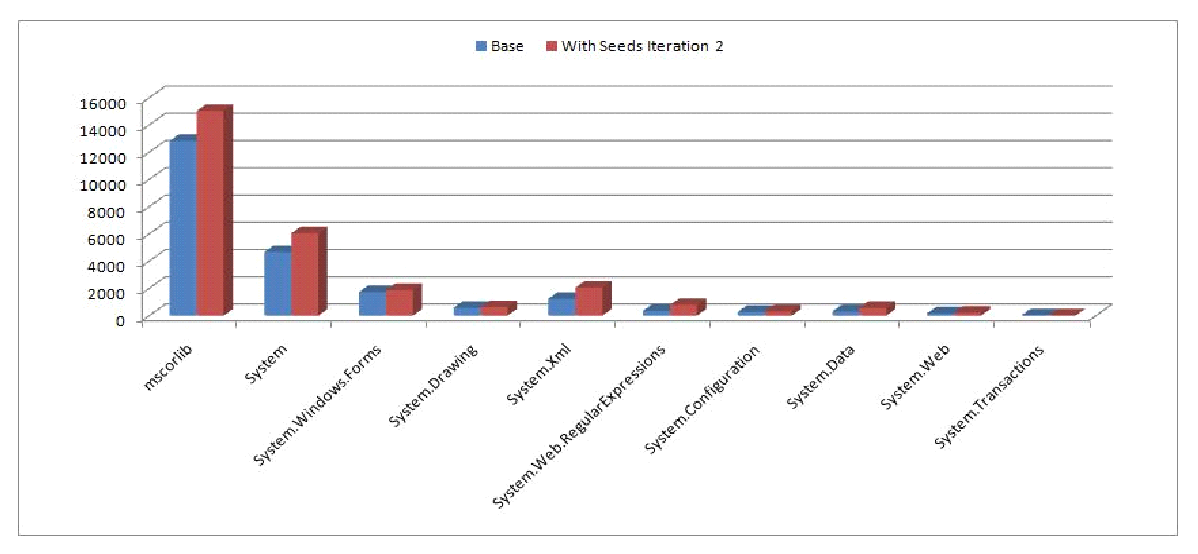
\includegraphics[scale=0.70,clip]{figs/RQ2_1.eps}\vspace*{-1ex}
%\caption{Comparison of base coverage and coverage achieved by regression tests of Mode 4 (WithSeeds Iteration 2).} \label{fig:rq2}
%\end{figure*}

%---------------------------------------------------------------------------------------
\subsection{Research Questions}
\label{sec:research}

We address the following three research questions in our evaluations.

\begin{itemize}
\item RQ1: Can our approach handle large real-world applications in automatically generating regression tests that achieve a high coverage of the code under test? 
\item RQ2: Do seed tests help achieve higher coverage of the code under test than without using seed tests?
\item RQ3: Can more machine power help generate new regression tests that can achieve more coverage of the code under test?
\end{itemize}

%---------------------------------------------------------------------------------------
\subsection{Subject Applications}

We used two core .NET 2.0 framework base class libraries as subject applications in our evaluations. We selected these libraries because these libraries are shipped and maintained in different distributions such as Version 2 and Version 4 of the ``desktop CLR'', 32-bit/64-bit Silverlight, and .NET compact framework. Therefore, it is paramount for the .NET product group to maintain identical behavior and detect any new defects between different versions of these base class libraries. Table~\ref{tab:subjects} shows the two libraries (mscorlib and System) used in our evaluations and their characteristics such as the number of classes and methods. The table also shows statistics of eight other libraries of .NET 2.0 framework. Although these other eight libraries are not our primary targets for generating regression tests, our generated regression tests include methods from these libraries since these libraries are developed based on the two core libraries: mscorlib and System. In our evaluations, we use these additional eight libraries also while presenting our coverage results. The table shows that these libraries include $0$ LOC with $0$ classes and $0$ methods.

\setlength{\tabcolsep}{1pt}
\begin{table}[t]
\begin{SmallOut}
\begin{CodeOut}
\begin{center}
\begin {tabular} {|l|c|c|c|}
\hline
\textbf{.NET libraries} & \textbf{LOC} & \textbf{\# public} & \textbf{\# public}\\ 
 & & \textbf{classes} & \textbf{methods}\\ 
\hline
\hline  mscorlib & 185K & 1440 & 17800 \\
\hline  System & & & \\
\hline  System.Windows.Forms & & & \\
\hline  System.Drawing & & & \\
\hline  System.Xml & 150K & 686 & 9920 \\
\hline  System.Web.RegularExpressions & & & \\
\hline  System.Configuration & & & \\
\hline  System.Data & 196K & 648 & 11550 \\
\hline  System.Web &  & & \\
\hline  System.Transactions & & & \\
\hline \textbf{TOTAL} &  &  &   \\
\hline
\end{tabular}
\end{center}
\end{CodeOut}
\end{SmallOut}\vspace*{-4ex}
\centering \caption {\label{tab:subjects}Ten .NET framework base class libraries used in our evaluations}
\end{table}

%---------------------------------------------------------------------------------------
\subsection{Evaluation Setup}

In our approach, we used nine machines that can be classified into three configuration categories. On each machine, we launched multiple Pex processes. The number of processes launched on a machine is based on the configuration of the machine. For example, on an eight core machine, we launched seven Pex processes. Each Pex process was exploring one class (including multiple PUTs) at a time. Table~\ref{tab:mconfig} shows all three configuration categories. The table also shows the number of machines of each configuration and the number of Pex processes launched on each machine.

\setlength{\tabcolsep}{1pt}
\begin{table}[t]
\begin{SmallOut}
\begin{CodeOut}
\begin{center}
\begin {tabular} {|l|c|c|}
\hline
\textbf{Machine Configuration} & \textbf{\# of} & \textbf{\# of} \\  
 & \textbf{machines} & \textbf{processes}\\  
\hline
\hline  Xeon 2 CPU @ 2.50 GHz, 8 cores & 1 & 7\\
				16 GB RAM & & \\
\hline  Quad core 2 CPU @ 1.90 GHz, 8 cores& 2 & 7\\
				8 GB RAM & & \\
\hline  Intel Xeon CPU @2.40 GHz, 2 cores& 6 & 1\\
				1 GB RAM & & \\
\hline
\end{tabular}
\end{center}
\end{CodeOut}
\end{SmallOut}\vspace*{-4ex}
\centering \caption {\label{tab:mconfig}Three categories of machine configurations used in our evaluations.}
\end{table}

As we used .NET framework base class libraries in our evaluations, the generated tests may invoke method calls that can can cause external side effects, and change the machine configuration. Therefore, while executing the code during exploration of PUTs or while running generated tests, we created a sand-box with the ``Internet'' security permission. This permission represents the default policy permission set for the content from an unknown origin. This permission blocks all operations that involve environment interactions such as file creations or registry accesses by throwing \CodeIn{SecurityException}. Since we use sand-box in our evaluations, the reported coverage is lower than the actual coverage that can be achieved by our generated regression tests.

To address our research questions, we first created a base line in terms of the code coverage achieved by the seed tests, referred to as \emph{base coverage}. In our evaluations, we use block coverage (Section~\ref{sec:blockcov}) as a coverage criteria. We report our coverage in terms of the number of blocks covered in the code under test. We don't give an upper bound on the number of reachable basic blocks, as we don't know which blocks are actually reachable from the given scenarios.

We next generated regression tests in four different modes. In Mode 1 (referred to as \emph{WithoutSeeds Iteration 1}), we generated regression tests without using seed tests for one iteration. In Mode 2 (referred to as \emph{WithoutSeeds Iteration 2}), we generated regression tests without using seed tests for two iterations. The regression tests generated in Mode 2 are a super set of the regression tests generated in Mode 1. In Mode 3 (referred to as \emph{WithSeeds Iteration 1}), we generated regression tests with using seed tests for one iteration. Finally, in Mode 4 (referred to as \emph{WithSeeds Iteration 2}), we generated regression tests with using seed tests for two iterations. Modes 1 and 3 took one and half day for generating tests, whereas Modes 2 and 4 took three days since these modes correspond to Iteration 2.

\setlength{\tabcolsep}{1pt}
\begin{table}[t]
\begin{SmallOut}
\begin{CodeOut}
\begin{center}
\begin {tabular} {|l|c|c|c|}
\hline
\textbf{Mode} & \textbf{\# of} & \textbf{\# of covered} & \textbf{\% of increase}\\  
 & \textbf{Tests} & \textbf{blocks} & \textbf{from base}\\  
\hline
\hline  WithoutSeeds Iteration 1 & 248,306 & 21,920 & 0\%\\
\hline  WithoutSeeds Iteration 2 & 412,928 & 23,176 & 4.8\%\\
\hline  WithSeeds Iteration 1 & 376,367 & 26,939 & 21.8\%\\
\hline  WithSeeds Iteration 2 & 501,799 & 27,485 & 24.3\%\\
\hline
\end{tabular}
\end{center}
\end{CodeOut}
\end{SmallOut}\vspace*{-4ex}
\centering \caption {\label{tab:gentests}Generated regression tests.}
\end{table}

%---------------------------------------------------------------------------------------
\subsection{RQ1: Generated Regression Tests}

We next address the first research question of whether our approach can handle large real-world applications in automatically generating regression tests. This research question helps to show that our approach can be used in practice and can address scalability issues in generating regression tests for large applications. We first present the statistics after each phase in our approach and next present the number of regression tests generated in each mode.

In the capture phase, our approach recorded $\approx$1.50 GB C\# source code (including 433,809 traces) of dynamic traces for the two libraries. The average trace length includes $21$ method calls and the maximum trace length includes $52$ method calls. As our capture phase transforms each dynamic trace into a PUT and a seed test, the capture phase resulted in 433,809 PUTs and 433,809 seed tests. 

In the minimize phase, our approach uses static analysis to filter out duplicate PUTs. Our static analysis took 45 minutes and resulted in 68,575 unique PUTs. Our approach uses dynamic analysis to filter our duplicate seed tests. Our dynamic analysis took 5 hours and resulted in 128,185 unique seed tests. These results show that there are a large number of duplicate PUTs and seed tests, and show the significance of our minimize phase. We next measured the block coverage achieved by these 128,185 unique seed tests in the code under test and used this coverage as \emph{base coverage}. These tests covered 22,111 blocks in the code under test. 

Table~\ref{tab:gentests} shows the number of regression tests generated in each mode along with the number of covered blocks. The table also shows the percentage of increase
in the number of blocks compared to the base coverage. As shown in results, in Mode 4 (WithSeeds Iteration 2), our approach achieved 24.3\% higher coverage than the base coverage. Table~\ref{tab:detailedres} shows more detailed results of coverages achieved for all ten .NET libraries. Column ``.NET libraries'' shows the library under test. Column ``Base Coverage'' shows the number of blocks covered by seed tests for each library. Column ``WithOutSeeds Iteration 1'' shows the number of blocks covered (``\# blocks'') and the percentage of increase in the coverage (``\% increase'') with respect to the base coverage in this mode. Similarly, Columns ``WithOutSeeds Iteration 2'', ``WithSeeds Iteration 1'', and ``WithSeeds Iteration 2'' show the results of the other three modes. 

As we use seed tests during our exploration in Mode ``WithSeeds Iteration 2'', the coverage achieved is either the same or higher than the base coverage. However, our approach has achieved significant higher coverages than base coverage for libraries mscorlib and System (in terms of the number of additional blocks covered). The primary reason is that most of the classes in these libraries are stateless and do not require environment interactions. The results show that our approach can handle large real-world applications and can generate large number of regression tests that achieve a high coverage of the code under test.

\setlength{\tabcolsep}{1pt}
\begin{table*}[t]
\begin{SmallOut}
\begin{CodeOut}
\begin{center}
\begin {tabular} {|l|c|c|c|c|c|c|c|c|c|}
\hline
\textbf{.NET libraries} & \textbf{Base} & \multicolumn{2}{|c|}{\textbf{WithOutSeeds}} & \multicolumn{2}{|c|}{\textbf{WithOutSeeds}} & \multicolumn{2}{|c|}{\textbf{WithSeeds}} & \multicolumn{2}{|c|}{\textbf{WithSeeds}}\\ 
 & \textbf{Coverage} & \multicolumn{2}{|c|}{\textbf{Iteration 1}} & \multicolumn{2}{|c|}{\textbf{Iteration 2}} & \multicolumn{2}{|c|}{\textbf{Iteration 1}} & \multicolumn{2}{|c|}{\textbf{Iteration 2}}\\ 
\cline{3-10}
 & \# blocks & \# blocks & \% increase & \# blocks & \% increase & \# blocks & \% increase & \# blocks & \% increase\\ 
\hline  mscorlib   						& 12827 	& 13063 & 1.84		& 13620 & 6.18	& 14808	& 15.44		& 15018	& 17.08					\\
\hline  System    						& 4651  	& 4062  & -12.67	& 4243	& -8.77	& 5907	& 27.00		& 6039	& 29.84 				\\
\hline  System.Windows.Forms  & 1730 		& 1572  & -9.13		& 1774	& 2.54	& 1782	& 3.01		& 1865	& 7.80 					\\
\hline  System.Drawing 				& 570			& 580		& 1.75		& 591		& 3.68	& 618		& 8.42		& 625		& 9.65 					\\
\hline  System.Xml 						& 1229    & 1390	& 13.10		& 1462	& 18.96	& 1959	& 59.40		& 2045	& 66.40 				\\
\hline  System.Web.Regular 		& 351     & 330		& -5.98		& 520		& 48.15	& 754		& 114.81 	& 771		& 119.66 				\\
			  Expressions 					& 				& 			& 				& 			& 			& 			& 				& 			&  							\\
\hline  System.Configuration 	& 263 		& 297 	& 12.93		& 297		& 12.93	& 302		& 14.83		& 306		& 16.35 				\\
\hline  System.Data 					& 301 		& 380		& 26.25		& 422		& 40.20	& 562		& 86.71		& 569		& 89.04 				\\
\hline  System.Web 						& 154			& 211		& 37.01		& 212		& 37.66	& 212		& 37.66		& 212		& 37.66 				\\
\hline  System.Transactions 	& 35			& 35		& 0.00		& 35		& 0.00	& 35		& 0.00		& 35		& 0.00 					\\
\hline \textbf{TOTAL/AVERAGE} & \textbf{22111} & \textbf{21920} & \textbf{<0} & \textbf{23176} & \textbf{4.80} & \textbf{26939}	& \textbf{21.80} & \textbf{27485} & \textbf{24.30} \\
\hline
\end{tabular}
\end{center}
\end{CodeOut}
\end{SmallOut}
\centering \caption {\label{tab:detailedres}Comparison of coverages achieved for ten .NET libraries used in our evaluation.}
\end{table*}

%---------------------------------------------------------------------------------------
\subsection{RQ2: Using Seed Tests}

We next address the second research question of whether seed tests help achieve higher code coverage compared to without using seed tests. To address this question, we compare the coverages achieved by generated tests in Modes ``WithoutSeeds Iteration 2'' and ``WithSeeds Iteration 2''. As shown in Table~\ref{tab:detailedres}, Mode ``WithSeeds Iteration 2'' always achieved higher coverage than Mode ``WithoutSeeds Iteration 2''. On average ``WithSeeds Iteration 2'' achieved 18.6\% higher coverage than Mode ``WithoutSeeds Iteration 2''. The table also shows that there is a significant increase in the coverage achieved for the \CodeIn{System.Web.RegularExpressions} library. 
In Section~\ref{sec:explore}, we described one of the advantages of seed tests is that seed tests can help cover certain paths that are hard to be covered without using those tests. The \CodeIn{System.Web.RegularExpressions} library is an example for such paths since this library requires complex regular expressions to cover certain paths in the library. It is quite challenging for Pex or any other dynamic-symbolic-execution-based approach to generate concrete values that represent regular expressions. Therefore, concrete values in the seed tests helped achieve higher coverage for this library. In summary, the results show that seed tests help achieve higher coverages compared to without using seed tests.

%\begin{figure*}[t]
%\centering
%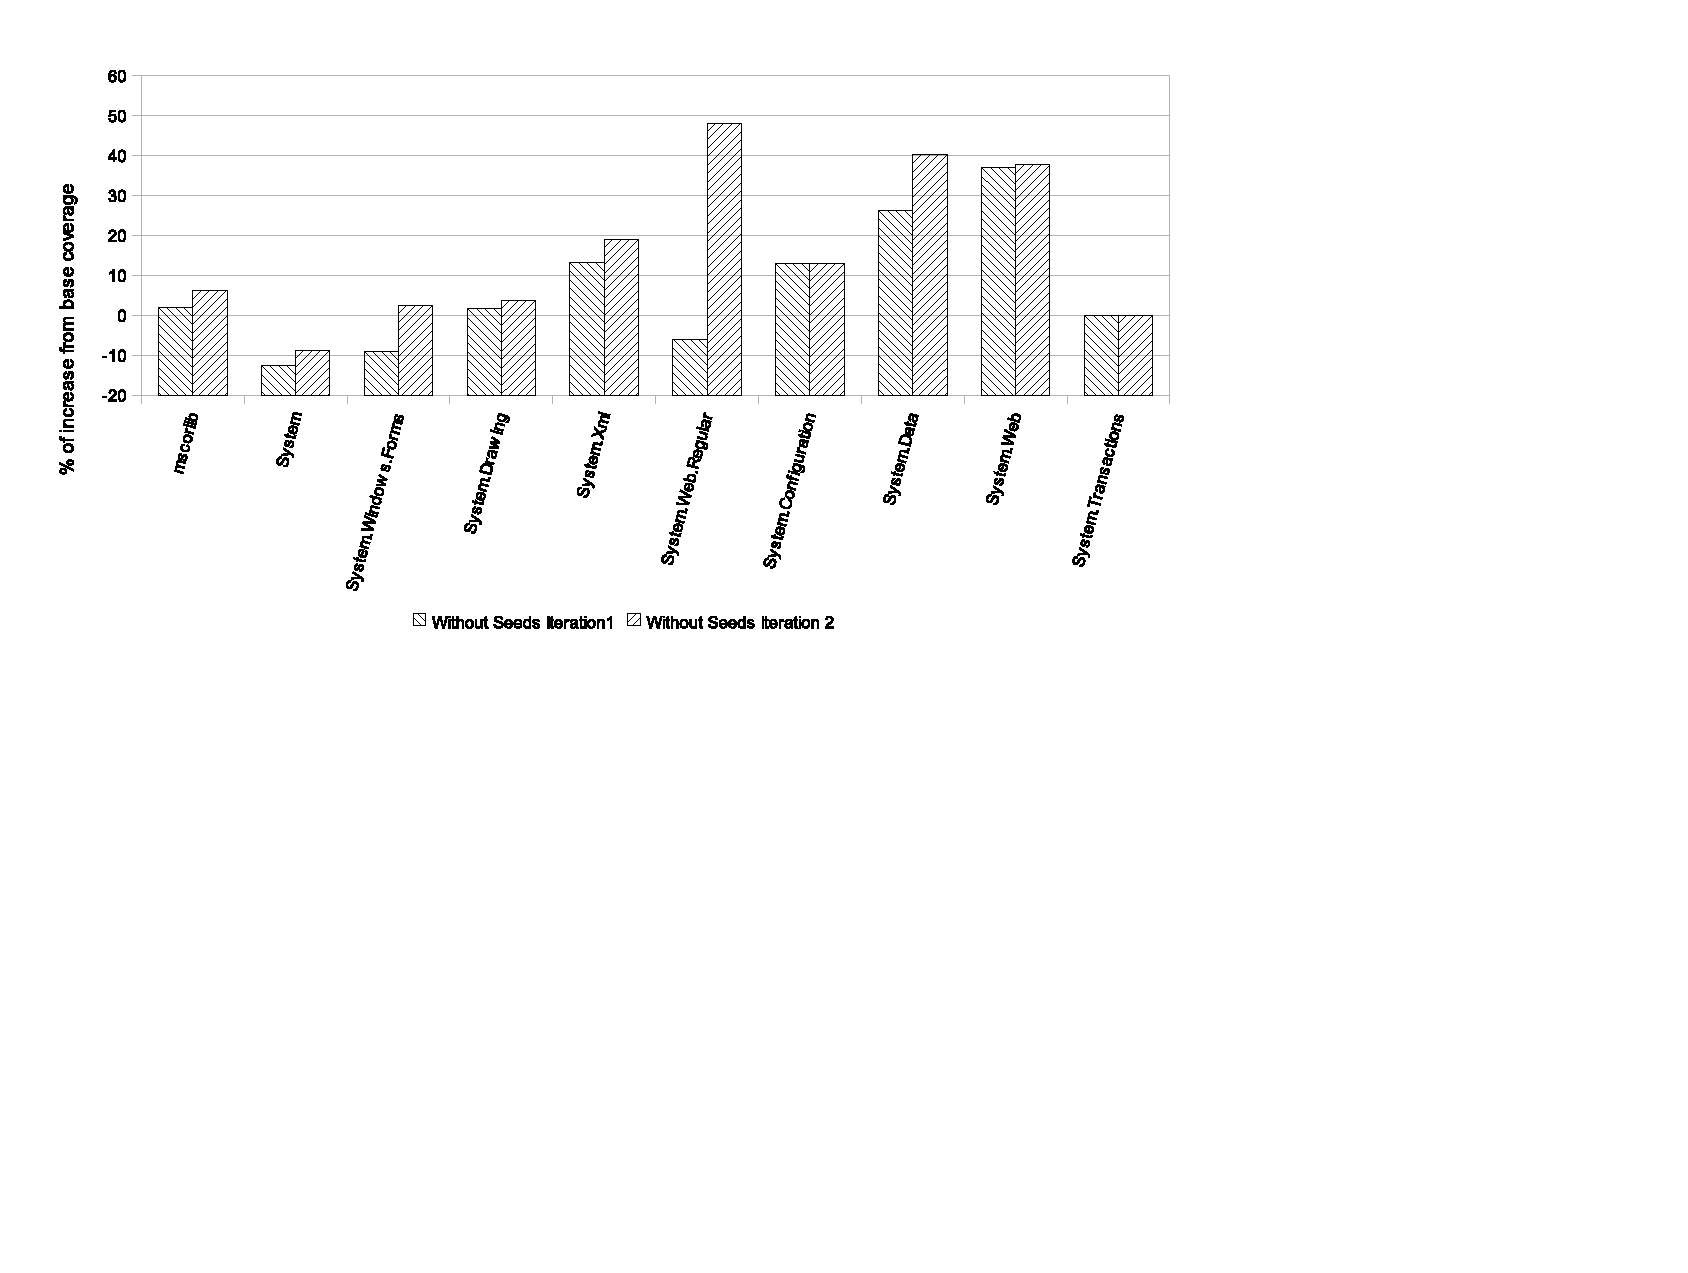
\includegraphics[scale=0.70,clip]{figs/RQ3_1.eps}\vspace*{-1ex}
%\caption{Comparison of code coverages achieved by base, Modes 2 (WithoutSeeds Iteration 2) and 4 (Withseeds Iteration 2).} \label{fig:rq3}
%\end{figure*}

%---------------------------------------------------------------------------------------
\subsection{RQ3: Using More Machine Power}

We next address the third research question of whether more machine power helps to achieve more coverage. This research question helps to show that additional coverage can be achieved in further iterations of our approach. To address this question, we compare coverages achieved in Mode ``WithoutSeeds Iteration 1'' with Mode ``WithoutSeeds Iteration 2'', and Mode ``WithSeeds Iteration 2'' with Mode ``WithSeeds Iteration 2'' (shown in Table~\ref{tab:detailedres}). 

On average, Mode ``WithoutSeeds Iteration 2'' achieved 5.73\% higher coverage than Mode 1. This result show that our approach can achieve additional coverage in further iterations. However, the coverage from Mode 1 to Mode 2 is not doubled. The primary reason is that it gets harder to cover new blocks in further iterations.

Figure~\ref{fig:rq42} shows the comparison results of Mode 3 with Mode 4. On average, Mode 4 achieved 2.0\% higher coverage than Mode 3. As shown, the increase in coverage from Mode 3 to Mode 4 is less than the increase in the coverage from Mode 1 to Mode 2. This difference is due to seed tests that help achieve higher coverage during Mode 3, leaving more harder blocks to be covered in Mode 4. In summary, the results show that further iterations can help generate new regression tests that can achieve more coverage.

\begin{figure*}[t]
\centering
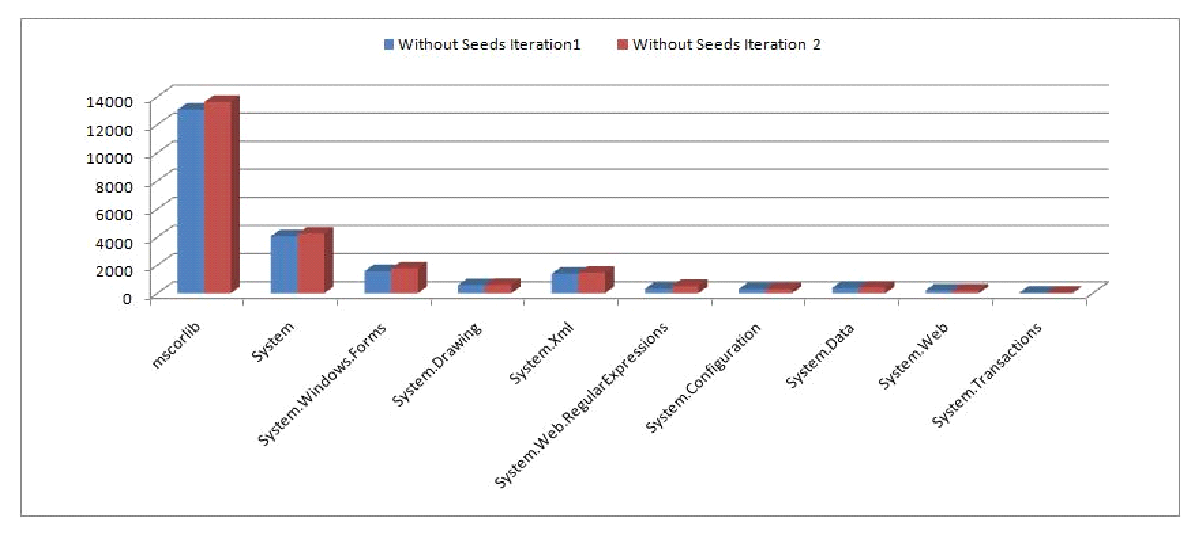
\includegraphics[scale=0.70,clip]{figs/RQ4_1_1.eps}\vspace*{-1ex}
\caption{\label{fig:rq41}Comparison of code coverages achieved by Modes 1 (WithoutSeeds Iteration 1) and 2 (WithoutSeeds Iteration 2).} 
\end{figure*}


\begin{figure*}[t]
\centering
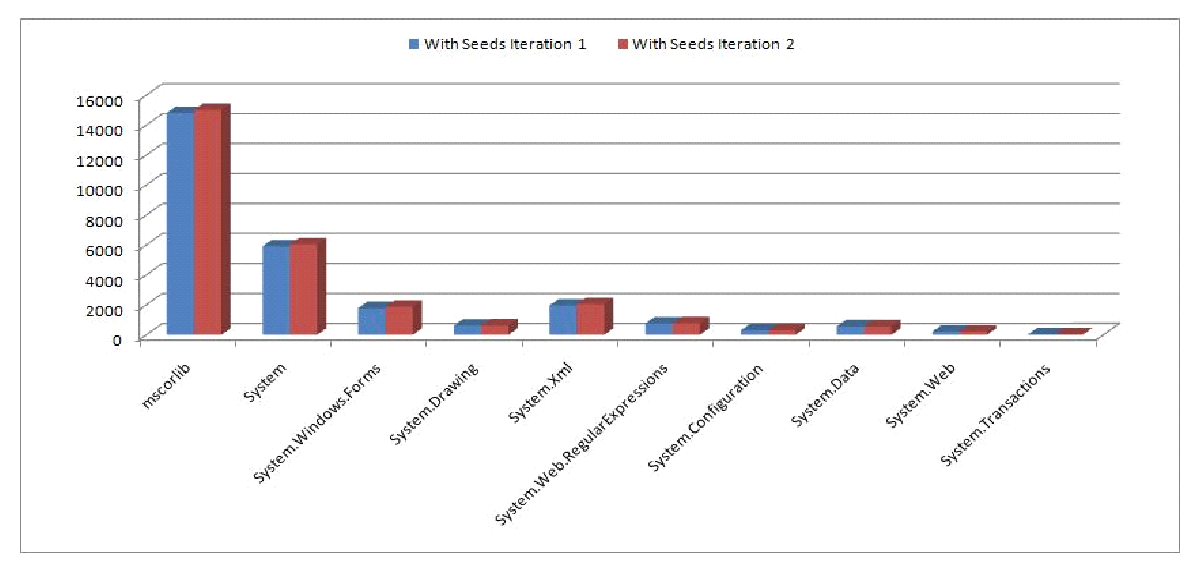
\includegraphics[scale=0.70,clip]{figs/RQ4_2_1.eps}\vspace*{-1ex}
\caption{\label{fig:rq42}Comparison of code coverages achieved by Modes 3 (WithSeeds Iteration 1) and 4 (Withseeds Iteration 2).}
\end{figure*}


%---------------------------------------------------------------------------------------
%\subsection{Real Defects}

%Our approach automatically generates test scenarios from dynamic traces. We use these test scenarios
%in generating PUTs and then generating regression tests on a stable versions. These regression tests
%can be used on future versions to detect regression faults. In our approach, we cannot detect
%defects in the version on which regression tests generated because of lack of test oracles. However,
%we identify that many exceptions are observed while generating regression tests on the version.
%We next describe the raised exceptions and describe more about the defects detected.
\section{Threats to Validity}
\label{sec:threats}
The threats to external validity primarily include the degree to which the subject programs and used CSE are representative of true practice. The current subjects range from small-scale libraries such as Java SQL APIs to large-scale libraries such as BCEL and Hibernate. We used only one CSE, i.e., Google code search, which is a well-known CSE. These threats could be reduced by more experiments on wider types of subjects and by using other CSEs in future work. The threats to internal validity are instrumentation effects that can bias our results. Faults in our Alattin prototype might cause such effects. There can be errors in our inspection of source code for confirming rules or defects. To reduce these threats, we inspected available specifications and also call sites in source code.
\section{Discussion and Future Work}
\label{sec:future}

Although random and DSE-based approaches show considerable increase in branch coverage with the assistance from our approach, overall coverage achieved by these approaches are still not close to 100\% coverage. The reason is that often code under test includes complex branches that are quite difficult to cover. We next give an example of a difficult branch that is not covered by any of the approaches used in our evaluation. We use the code example shown in Figure~\ref{fig:diffbranch} as an illustrative example. This difficult branch is in the \CodeIn{Visit} method of the \CodeIn{BreadthFirstSearchAlgorithm} class. The receiver-object state to reach Statement 8 requires that the \CodeIn{VisitedGraph} object has a non-empty set of vertices and edges. Reaching Statement 8 also requires a specific object state for the argument \CodeIn{s}. In particular, the vertex represented by the argument \CodeIn{s} should already exist in the \CodeIn{VisitedGraph} object and should have outgoing edges. Although our extracted sequences include a sequence for achieving a desirable receiver-object state, our sequences do not include a necessary sequence for achieving a desirable argument-object state. In future work, we plan to further address these issues by generating new sequences using evolutionary approaches~\cite{tonella:etoc,  inkumsah08:improving}. There, we can use our extracted sequences as an initial set for these evolutionary approaches to evolve. Generation of new sequences using evolutionary approaches can also help reduce the bias in our approach, where our approach gives more preference to verify common usage rather than uncommon usage.

\begin{figure}[t]
\begin{CodeOut}
\begin{alltt}
00:public void Visit(IVertex s) \{
01:\hspace*{0.1in}...
02:\hspace*{0.1in}m\_Q.Push(s);
03:\hspace*{0.1in}while (m\_Q.Count != 0) \{
04:\hspace*{0.2in}IVertex u = (IVertex)m\_Q.Peek(); 
05:\hspace*{0.2in}m\_Q.Pop();
06:\hspace*{0.2in}...
07:\hspace*{0.2in}foreach(IEdge e in VisitedGraph.OutEdges(u)) \{ 
08:\hspace*{0.3in}...		//Difficult branch
09:\hspace*{0.2in}\} 
10:\hspace*{0.1in}\}
11:\}
\end{alltt}
\end{CodeOut}\vspace*{-5ex}
\Caption{\label{fig:diffbranch} An example difficult branch not reached by any approach used in our evaluation.}\vspace*{-5ex}
\end{figure}

In our evaluations, for the \CodeIn{facebook} and \CodeIn{facebook.Utility} namespaces, branch coverage achieved by Randoop (with the assistance of our approach) is lower than branch coverage achieved by the test code (commonly written by  application developers). There are two primary reasons for lower coverage of these namespaces: limitations of the random mechanism of Randoop and our current implementation. Our current implementation does not handle several features such as inheritance or C\# generics. Therefore, our implementation could not capture some sequences due to their use of these features. In future work, we plan to extend our implementation to support these features. 

%In our current approach, gathering sequences is loosely coupled with dynamic symbolic execution. For example, we identify the target classes and gather method-call sequences from code bases. We next verify whether these sequences can help achieve the $\theta$ states. Therefore, some collected sequences can be irrelevant. In future work, we plan to identify a desirable target (such as a branch) that is not achieved by the dynamic symbolic execution and use that information to gather sequences. This additional information can help gather more relevant sequences. 

Our approach extracts sequences from code bases using the receiver or argument object types of a MUT (in a framework under analysis) and generates method bodies to assist test-generation approaches. Sometimes, these sequences may include object types specific to the code bases. For example, these object types can be classes that implement interfaces provided by the framework under analysis. In such scenarios, the method bodies generated by our approach are not compilable. Currently, we fix those compilation errors manually. In future work, we plan to automatically compile and verify extracted sequences to reduce this manual effort.

\Comment{We currently gather \emph{only} one path from a CFG to generate sequences. However, there can be different sequences
across multiple paths in the CFG. In future work, we plan to collect sequences from multiple paths in the CFG. We also plan to develop clustering heuristics to cluster similar sequences.}


\section{Related Work}
\label{sec:related} In this section, we introduce related work and
discuss our contributions.

\textbf{Language migration.} It is a research topic with a long
history to migrate projects of one language into other
languages~\cite{samet1981experience}. To reduce the human effort of
language migration, researchers propose various approaches to
automate the
process~\cite{van1999identifying,waters1988program,mossienko2003automated,yasumatsu1995spice,hainaut2008migration}.
Most of these approaches focus the syntax differences among
languages. For example, Deursen \emph{et
al.}~\cite{van1999identifying} propose an approach to identify
objects in legacy code, and the results are useful to deal with the
difference  between object-oriented languages and procedural
languages. As shown by El-Ramly \emph{et
al.}~\cite{el2006experiment}'s experience report, existing
approaches and tools support only a subset of APIs, and consequently
it becomes an important to automate API transformation. Our approach
mines API mapping among languages to aid language migration,
complementing the preceding approaches.

\textbf{Library migration.} With the evaluation of libraries, some
APIs may become incompatible. To deal with the problem, some
approaches have been proposed. In particular, Henkel and
Diwan~\cite{henkel2005catchup} propose an approach that captures and
replay API refracturing actions to keep client code updated. Xing
and Stroulia~\cite{xing2007api} propose an approach that recognizes
the changes of APIs by comparing the differences of two versions of
libraries. Balaban \emph{et al.}~\cite{balaban2005refactoring}
propose an approach to help translate client code when mapping
relations of libraries are available. Different from these
approaches, our approach focuses on mapping relations of APIs among
different languages. In addition, as our approach uses ATGs to mine
mapping relations of APIs, our approach helps mine mapping relations
for those API methods whose input orders is changed or whose
functionalities are split into several methods if our approach is
applied in library migration.

\section{Conclusion}
\label{sec:conclusion}

Mapping relations of APIs are quite useful for the translation
of projects from one language to another language, and
it is difficult to mine these mapping relations due to various
challenges. In this paper, we propose a novel approach that mines mapping
relations of APIs from existing projects with multiple versions in
different languages. We conducted two evaluations to show the effectiveness
of our approach. The results show that our approach mines many API mapping
relations between Java and C\#, and these relations improve existing language
translation tools such as Java2CSharp.


\section*{Acknowledgments}

We thank Shuvendu Lahiri and Thomas Ball for sharing Randoop used in our evaluations.

\bibliographystyle{abbrv}
\begin{thebibliography}{10}

\bibitem{acharya06:mining}
M.~Acharya, T.~Xie, and J.~Xu.
\newblock {Mining Interface Specifications for Generating Checkable Robustness
  Properties}.
\newblock In {\em Proc. ISSRE}, pages 311--320, 2006.

\bibitem{agarwal:association}
R.~Agrawal and R.~Srikant.
\newblock Fast algorithms for mining association rules in large databases.
\newblock In {\em Proc. VLDB}, pages 487--499, 1994.

\bibitem{Clarke:symbolic}
L.~Clarke.
\newblock {A System to Generate Test Data and Symbolically Execute Programs}.
\newblock {\em IEEE Trans. Softw. Eng.}, 2(3):215--222, 1976.

\bibitem{thomas:algos}
T.~H. Cormen, C.~Stein, R.~L. Rivest, and C.~E. Leiserson.
\newblock {\em Introduction to Algorithms}.
\newblock McGraw-Hill Higher Education, 2001.

\bibitem{csallner:jcrasher}
C.~Csallner and Y.~Smaragdakis.
\newblock {JC}rasher: an automatic robustness tester for {J}ava.
\newblock {\em Softw. Pract. Exper.}, 34(11):1025--1050, 2004.

\bibitem{random:duran}
J.~Duran and M.~Ntafos.
\newblock An evaluation of random testing.
\newblock {\em IEEE Trans. Softw. Eng.}, 10(4):438--444, 1984.

\bibitem{Elbaum:capture}
S.~Elbaum, H.~N. Chin, M.~B. Dwyer, and J.~Dokulil.
\newblock {Carving differential unit test cases from system test cases}.
\newblock In {\em Proc. FSE}, pages 253--264, 2006.

\bibitem{Engler2001deviant}
D.~Engler, D.~Y. Chen, S.~Hallem, A.~Chou, and B.~Chelf.
\newblock {Bugs as deviant behavior: a general approach to inferring errors in
  systems code}.
\newblock In {\em Proc. SOSP}, pages 57--72, 2001.

\bibitem{FACEBOOK}
Facebook developer toolkit, 2008.
\newblock \url{http://www.codeplex.com/FacebookToolkit}.

\bibitem{godefroid:dart}
P.~Godefroid, N.~Klarlund, and K.~Sen.
\newblock {DART}: {D}irected automated random testing.
\newblock In {\em Proc. PLDI}, pages 213--223, 2005.

\bibitem{inkumsah08:improving}
K.~Inkumsah and T.~Xie.
\newblock Improving structural testing of object-oriented programs via
  integrating evolutionary testing and symbolic execution.
\newblock In {\em Proc. ASE}, pages 297--306, 2008.

\vfill\eject

\bibitem{JTEST}
Parasoft. {J}test manuals version 5.1. {O}nline manual, 2006.
\newblock \url{http://www.parasoft.com}.

\bibitem{khurshid:symbolic}
S.~Khurshid, C.~S. Pasareanu, and W.~Visser.
\newblock {Generalized symbolic execution for model checking and testing}.
\newblock In {\em Proc. TACAS}, pages 553--568, 2003.

\bibitem{king:symex}
J.~C. King.
\newblock {Symbolic Execution and Program Testing}.
\newblock {\em Communications of the ACM}, 19(7):385--394, 1976.

\bibitem{koushik:cute}
S.~Koushik, M.~Darko, and A.~Gul.
\newblock {CUTE: a concolic unit testing engine for C}.
\newblock In {\em Proc. ESEC/FSE}, pages 263--272, 2005.

\bibitem{Xiyang:fitness}
X.~Liu, H.~Liu, B.~Wang, P.~Chen, and X.~Cai.
\newblock {A unified fitness function calculation rule for flag conditions to
  improve evolutionary testing}.
\newblock In {\em Proc. ASE}, pages 337--341, 2005.

\bibitem{orso:capture}
A.~Orso and B.~Kennedy.
\newblock {Selective capture and replay of program executions}.
\newblock {\em SIGSOFT Softw. Eng. Notes}, 30(4):1--7, 2005.

\bibitem{pacheco:eclat}
C.~Pacheco and M.~D. Ernst.
\newblock Eclat: Automatic generation and classification of test inputs.
\newblock In {\em Proc. ECOOP}, pages 504--527, 2005.

\bibitem{pacheco:feedback}
C.~Pacheco, S.~K. Lahiri, M.~D. Ernst, and T.~Ball.
\newblock Feedback-directed random test generation.
\newblock In {\em Proc. ICSE}, pages 75--84, 2007.

\bibitem{QUICKGRAPH}
{QuickGraph: A 100\% C\# graph library with Graphviz Support, Version 2.0},
  2008.
\newblock \url{http://www.codeproject.com/KB/miscctrl/quickgraph.aspx}.

\bibitem{david:java}
D.~Saff, S.~Artzi, J.~H. Perkins, and M.~D. Ernst.
\newblock {Automatic test factoring for Java}.
\newblock In {\em Proc. ASE}, pages 114--123, 2005.

\bibitem{song07:unitplus}
Y.~Song, S.~Thummalapenta, and T.~Xie.
\newblock {UnitPlus}: Assisting developer testing in eclipse.
\newblock In {\em Proc. ETX}, pages 26--30, 2007.

\bibitem{thummalapenta07:parseweb}
S.~Thummalapenta and T.~Xie.
\newblock {PARSEWeb}: A programmer assistant for reusing open source code on
  the web.
\newblock In {\em Proc. ASE}, pages 204--213, 2007.

\bibitem{thummalapenta09:mining}
S.~Thummalapenta and T.~Xie.
\newblock {M}ining exception-handling rules as sequence association rules.
\newblock In {\em Proc. ICSE}, pages 496--506, 2009.

\bibitem{tillman:pexwhite}
N.~Tillmann and J.~de~Halleux.
\newblock Pex white box test generation for .{NET}.
\newblock In {\em Proc. TAP}, pages 134--153, 2008.

\bibitem{tillmann05:parameterized}
N.~Tillmann and W.~Schulte.
\newblock {Parameterized Unit Tests}.
\newblock In {\em Proc. ESEC/FSE}, pages 253--262, 2005.

\bibitem{tonella:etoc}
P.~Tonella.
\newblock Evolutionary testing of classes.
\newblock In {\em Proc. ISSTA}, pages 119--128, 2004.

\bibitem{wang:bide}
J.~Wang and J.~Han.
\newblock {BIDE}: Efficient mining of frequent closed sequences.
\newblock In {\em Proc. ICDE}, pages 79 -- 88, 2004.

\bibitem{wasylkowski07:detecting}
A.~Wasylkowski, A.~Zeller, and C.~Lindig.
\newblock Detecting object usage anomalies.
\newblock In {\em Proc. ESEC/FSE}, pages 35--44, 2007.

\bibitem{xie:rostra}
T.~Xie, D.~Marinov, and D.~Notkin.
\newblock Rostra: A framework for detecting redundant object-oriented unit
  tests.
\newblock In {\em Proc. ASE}, pages 196--205, 2004.

\end{thebibliography}
\end{document}
